% 电场强度叠加原理
%电场力/电荷/矢量叠加原理
% 和 “电场” 重复, 待删除. 例题可以加入到 “电场” 中

电场力是矢量,服从矢量叠加原理.即,如果在$F_1$,$F_2$,...,$F_k$分别表示点电荷$q_1$,$q_2$,...,$q_k$单独存在时电场施于空间同一点上试探电荷$q_0$的力.则它们同时存在时,电场施于该点试探电荷的力为$F_1$,$F_2$,...,$F_k$的矢量和,即
\begin{equation}
F = F_1 +F_2 +...+F_k
\end{equation}
由于库仑定律:
\begin{equation}
  F = Eq
\end{equation}
因此将上式(1)除以$q_0$,我们得到: 
\begin{equation}
E = E_1 + E_2 + ... +E_k
\end{equation}
其中$E_i = F_i/q_0$      ($i=1, 2, 3, 4, ...$)
因此我们可以得到:\textbf{点电荷组所产生的电场在某点的场强等于各点电荷单独存在时所产生的电场在该点场强的矢量叠加, 这个就叫做电场强度叠加原理,简称场强叠加原理.}


例题(如图 1所示)
\begin{figure}[ht]
\centering
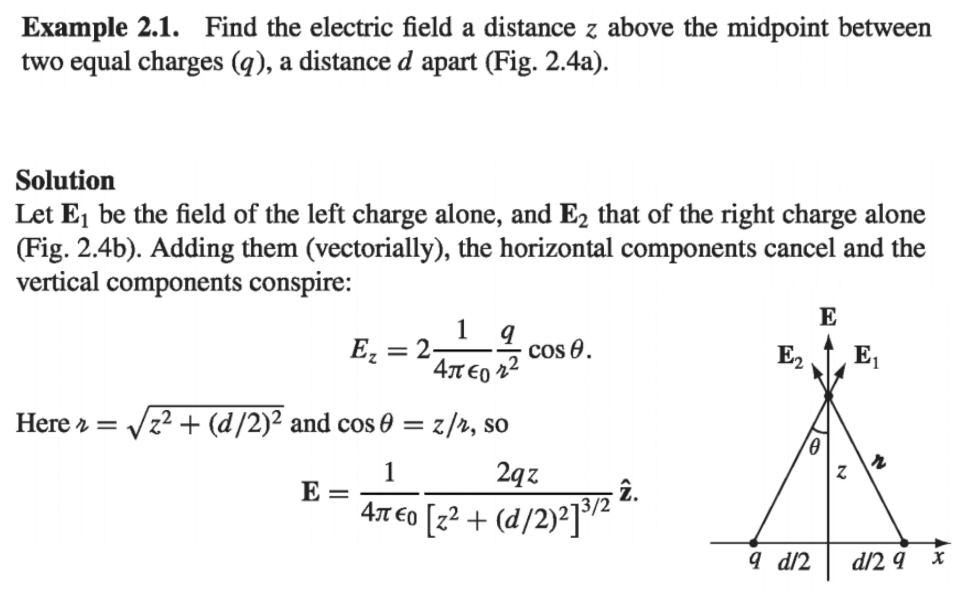
\includegraphics[width=14.25cm]{./figures/EleAdd_1.png}
\caption{电场叠加原理的例题} \label{EleAdd_fig1}
\end{figure}
